%% LyX 2.0.0 created this file.  For more info, see http://www.lyx.org/.
%% Do not edit unless you really know what you are doing.
\documentclass[english,traditabstract]{aa}
\usepackage[varg]{txfonts}
%\usepackage[english,brazilian]{babel}
\usepackage[T1]{fontenc}
\setcounter{tocdepth}{3}
\usepackage{prettyref}
\usepackage{array}
\usepackage{rotating}
\usepackage{float}
\usepackage{multirow}
\usepackage{amstext}
\usepackage{graphicx}
\usepackage{epstopdf}
\usepackage{subfigure}
\usepackage{gensymb}
\usepackage{longtable}
\usepackage{color}
%\usepackage{setspace}
%
%\usepackage{etoolbox}
%\AtBeginEnvironment{longtable}{\singlespacing}
%\setlength{\LTcapwidth}{\linewidth}


\makeatletter

%%%%%%%%%%%%%%%%%%%%%%%%%%%%%% LyX specific LaTeX commands.
%% Because html converters don't know tabularnewline
\providecommand{\tabularnewline}{\\}

%%%%%%%%%%%%%%%%%%%%%%%%%%%%%% User specified LaTeX commands.
\usepackage{natbib,twoopt}
\usepackage[breaklinks=true]{hyperref} %% to avoid \citeads line fills
\usepackage{arydshln}
\bibpunct{(}{)}{;}{a}{}{,} %% natbib format for A&A and ApJ
\makeatletter
\newcommandtwoopt{\citeads}[3][][]{\href{http://adsabs.harvard.edu/abs/#3}%
{\def\hyper@linkstart##1##2{}%
\let\hyper@linkend\@empty\citealp[#1][#2]{#3}}}
\newcommandtwoopt{\citepads}[3][][]{\href{http://adsabs.harvard.edu/abs/#3}%
{\def\hyper@linkstart##1##2{}%
\let\hyper@linkend\@empty\citep[#1][#2]{#3}}}
\newcommandtwoopt{\citetads}[3][][]{\href{http://adsabs.harvard.edu/abs/#3}%
{\def\hyper@linkstart##1##2{}%
\let\hyper@linkend\@empty\citet[#1][#2]{#3}}}
\newcommandtwoopt{\citeyearads}[3][][]%
{\href{http://adsabs.harvard.edu/abs/#3}
{\def\hyper@linkstart##1##2{}%
\let\hyper@linkend\@empty\citeyear[#1][#2]{#3}}}
\makeatother
\titlerunning{Predictions of stellar occultations by irregular satellites}
\authorrunning{Gomes-Júnior et al.}

\makeatother


\begin{document}

\title{Predictions of stellar occultations of 9 irregular satellites of giant planets
%\fnmsep\thanks{Table 8 are only available in electronic form at the CDS via anonymous ftp to cdsarc.u-strasbg.fr (130.79.128.5) or via http://cdsweb.u-strasbg.fr/cgi-bin/qcat?J/A+A/ and IAU NSDC data base at www.imcce.fr/nsdc.}
%\fnmsep\thanks{The complete version of Table 8 is available through CDS and IAU NSDC data base at www.imcce.fr/nsdc.}
%\fnmsep\thanks{Partially based on observations made at Laborat\'orio Nacional de Astrof\'{\i}sica (LNA), Itajub\'a-MG, Brazil.}
%\fnmsep\thanks{Partially based on observations through the ESO runs 079.A-9202(A), 075.C-0154, 077.C-0283 and 079.C-0345.}
%\fnmsep\thanks{\textbf{Partially based on observations made at Observatoire de Haute Provence (OHP), F-04870 Saint-Michel l'observatoire, France}}
}

\author{ A. R. Gomes-Júnior
          \inst{1},
          M. Assafin 
          \inst{1} \fnmsep\thanks{Affiliated researcher at Observatoire de Paris/IMCCE, 77 Avenue Denfert Rochereau 75014 Paris, France},
          R. Vieira-Martins
          \inst{1,2,3} \fnmsep\thanks{Affiliated researcher at Observatoire de Paris/IMCCE, 77 Avenue Denfert Rochereau 75014 Paris, France},
%          J.-E. Arlot
%          \inst{4},      
          J. I. B. Camargo
          \inst{2,3},     
%          F. Braga-Ribas
%          \inst{2,4}, 
%          D. N. da Silva Neto
%          \inst{6},
%          A. H. Andrei
%          \inst{1,2} \fnmsep\thanks{Affiliated researcher at Observatoire de Paris/SYRTE, 77 Avenue Denfert Rochereau, 75014 Paris, France},
          B. E. Morgado
          \inst{1},
%          A. Dias-Oliveira
%          \inst{2},
%          G. Benedetti-Rossi
%          \inst{2},
%          Y. Duchemin
%          \inst{4,7},
%          J. Desmars
%          \inst{4},
%          V. Lainey
%          \inst{4},
%          W. Thuillot
%          \inst{4}
          }

\offprints{A. R. Gomes-Júnior}

   \institute{Observatório do Valongo/UFRJ, Ladeira Pedro Antônio 43,
CEP 20.080-090 Rio de Janeiro - RJ, Brazil\\
              \email{altair08@astro.ufrj.br}
              \and
Observatório Nacional/MCT, R. General José Cristino 77,
CEP 20921-400 Rio de Janeiro - RJ, Brazil\\
              \email{rvm@on.br}
              \and
Laboratório Interinstitucional de e-Astronomia - LIneA, Rua Gal. José Cristino 77, Rio de Janeiro, RJ 20921-400, Brazil
%              \and
%Institut de mécanique céleste et de calcul des éphémérides - Observatoire %de Paris, UMR 8028 du CNRS,
%77 Av. Denfert-Rochereau, 75014 Paris, France\\
%              \email{arlot@imcce.fr}
%              \and
%Federal University of Technology - Paraná (UTFPR / DAFIS), Rua Sete de Setembro, 3165, CEP 80230-901, Curitiba, PR, Brazil
%              \and
%Centro Universitário Estadual da Zona Oeste, Av. Manual Caldeira de Alvarenga 1203, CEP 23.070-200 Rio de Janeiro RJ, Brazil
%              \and
%              ESIGELEC-IRSEEM, Technopôle du Madrillet, Avenue Galilée, 76801 Saint-Etienne du Rouvray, France
              }



\date{Received ; accepted }


\abstract
%{The irregular satellites of the giant planets are believed to have been captured during the evolution of the solar system. Knowing their physical parameters, such as size, density and albedo is important to constrain where they came from and how they were captured. The best way to obtain these parameters are observations in situ by spacecrafts or from stellar occultations by the objects. Both techniques demand that the orbits are well known.}
%{We aimed to obtain good astrometric positions of irregular satellites in order to improve their orbits and ephemeris.}
%{We identified and reduced observations of several irregular satellites from three databases containing more than 8000 images obtained between 1992 and 2014 at three sites (Observatório do Pico dos Dias, Observatoire de Haute-Provence and European Southern Observatory - La Silla).  We used the software PRAIA (Platform for Reduction of Astronomical Images Automatically) to make the astrometric reduction of the CCD frames. The UCAC4 catalogue represented the International Celestial Reference System in the reductions. The identification of the satellites in the frames was done through their ephemerides as determined from the SPICE/NAIF kernels. Some procedures were taken to overcome missing or incomplete information (coordinates, date), mostly for the older images.}
%{We managed to obtain more than 6000 positions for 18 irregular satellites, being 12 of Jupiter, 4 of Saturn, 1 of Uranus (Sycorax) and 1 of Neptune (Nereid). For some satellites the number of obtained positions is more than 50\% of that used in earlier orbital numerical integrations.}
%{Comparison of our positions with recent JPL ephemeris suggests the presence of systematic errors in the orbits for some of the irregular satellites. The most evident case was an error in the inclination of Carme.}


\keywords{Occultations - Planets and satellites: general - Planets and satellites: individual: Jovian and Saturnian irregular satellites}

\maketitle

\section{Introduction} \label{Sec: introducao} 

Irregular satellites, also known as outer satellites, of the giant planets are objects orbiting the planets from a distant, eccentric and highly inclined orbit, most of them are retrograde. Because of these peculiar orbits, it is largely accepted that these objects were captured by their planets in the early solar system \citep{Sheppard2005}.

There is a number of capture mechanisms of objects by giant planets proposed in the literature. There is the Gas Drag in the primordial circumplanetary nebulae \citep{Sheppard2005} where the object would be affected by the gas drag and its velocity slowed down until it be captured by the planet. Another mechanism is called pull-down capture \citep{Sheppard2005}, where the mass of the planet would increase while the object was temporarily captured. 

A mechanism based in the Nice model \citep{Morbidelli2005, Tsiganis2005, Gomes2005} was proposed by \cite{Nesvorny2007} and, in the specific case of Jupiter with the modern Nice model, by \citealp{Nesvorny2014}. During the early solar system instability, encounters between the outer planets occurred. These planetary encounters could exchange energy and angular momentum between planets and the objects nearby making it possible for the capture of irregular bodies by the giant planets. In this scenario, the survival rate of prior-LHB (Late Heavy Bombardment) satellites is very small.

Another important mechanism is the capture through collisional interactions \citep{Sheppard2005}. A collision between two small bodies in the Hill's sphere of the planet could generate fragmented objects and the dissipated energy could be such that some of these objects could be captured.

Some of these objects are in dynamical groups with similar orbital elements, called families, similar to families found in the Main Asteroid Belt. These families may have been created by a parent body disrupted by collisions with comets or other satellites \citep{Nesvorny2004}. Collisions with comets are more likely to have occurred during the Late Heavy Bombardment (LHB) \citep{Gomes2005}.

\cite{Nesvorny2003} studied the collision rates between irregular satellites and concluded that some satellites could have been removed by collision with a bigger satellite. The rate collision between satellites of the Himalia Group (Himalia, Elara, Lysithea and Leda, mainly), for instance, was found to be more than one during the solar system age suggesting that their current structure was originated by satellite-satellite collision.

For Phoebe, ejected material from its surface caused by impacts could evolve due to Poynting-Robertson drag and collide with Iapetus causing the large variation in albedo observed on it \citep{Nesvorny2003}. Indeed, Cassini was able to detected in Phoebe an absorption feature at 2.42 $\mu m$ (probably CN combinations) that was also detected in the dark side of Iapetus \citep{Clark2005}.

The region of origin of these object is not well known, \cite{Grav2003} and \cite{Grav2007} showed that the irregular satellites from the giant planest have their colors and spectral slopes similar to C-, D- and P-type asteroids, Centaurs and trans-neptunian objects (TNOs) suggesting that they have been originated from different locations in the early solar system.

In this work, we study these objects as possible representatives of the small TNOs population. TNOs are objects that due to their distance may be highly preserved having their properties similar to those they had when they were formed, then providing history and evolution of the outer solar system \citep{Camargo2013}. Due to their distance, the smaller objects from this region are more difficult to observe and study.

In the intent to obtain the physical parameters (size, shape, albedo, density, etc) of the irregular satellites and help identify their origin locations, we will make use of the stellar occultation technique. This technique is the best one to obtain these parameters of the solar system objects from ground-based observations providing more accurate results than other ground-based techniques \citep{Sicardy2011, Ortiz2012, Braga-Ribas2014}.

Since their estimated sizes are very small (see table \ref{} \textcolor{red}{Ainda vou fazer a tabela}), predict the exact location and instant where the shadow will cross the Earth demands a good precision. For instance, the bigger irregular satellite of Jupiter has an estimated size of 150 km \citep{Porco2003}, which is equivalent to an apparent size of 40 mas, must have an error smaller than its size for being observable. For the other objects, smaller or farther than Himalia, the situation is more difficult.

As pointed out by \cite{GomesJunior2015}, the ephemeris of the irregular satellites have errors that may reach 200 mas for some satellites. For an object at the distance of Jupiter, this represents an error bigger than 700 km in the shadow path.

We present in this paper the stellar occultation predictions for the 7 major irregular satellites of Jupiter (Himalia, Elara, Pasiphae, Lysithea, Carme, Ananke and Sinope), Phoebe from Saturn and Nereid from Neptune. In the section \ref{Sec: Rationale} we explore the scientific rationale for study the irregular satellites and the possibility of having a common origin with TNOs. In section \ref{Sec: Offset} we show the correction made to the ephemeris for better predict stellar occultations. In section \ref{Sec: predictions}, we present the predictions of the stellar occultations by irregular satellites and how they were made. Some test realized to confirm the predictions are presented in section \ref{Sec: testes} and the conclusion is given in section \ref{Sec: conclusions}.

\section{Scientific Rationale} \label{Sec: Rationale}

As explicited in section \ref{Sec: introducao}

%Because they are faint, the majority of these objects was discovered only in the last century\footnote{Website: http://ssd.jpl.nasa.gov/?sat\_discovery} . They were never visited by a spacecraft, with the exception of Himalia, Phoebe and Nereid, in a flyby by the Cassini space probe in 2000 for Himalia \citep{Porco2003} and in 2004 for Phoebe \citep{Desmars2013} and in a flyby by the Voyager 2 space probe in 1989 for Nereid \citep{Smith1989}. Even in situ, they were still opportunity target observations resulting in not optimal measurements, with size errors of $10 km$ for Himalia and $25 km$ for Nereid \citep{Thomas1991}. The exception is Phoebe with a very accurate measurement of size with a mean radius error of $0.7 km$ \citep{Thomas2010}.

%If these objects were captured, there remains the question of where they came from. \citealp{Clark2005} showed from imaging spectroscopy from Cassini that Phoebe has a surface probably covered by material from the outer solar system and \citealp{Grav2003} showed that the satellites of the Jovian Prograde Group Himalia have grey colors implying that their surfaces are similar to that of C-type asteroids. In that same work, the Jovian Retrograde Group Carme was found to have surface colors similar to the D-type asteroids like Hilda or Trojan families while JXIII Kalyke has a redder color like Centaurs or trans-neptunian objects (TNOs).

%For Saturnian satellites, \citealp{Grav2007} showed by their colors and spectral slopes that these satellites contain a more or less equal fraction of C-, P- and D-like objects but SXXII Ijiraq is marginally redder than D-type objects. These works may suggest different origins for the irregular satellites.

%In this context, we used 3 databases for deriving precise positions for the irregular satellites observed at Observatório do Pico dos Dias (1.6 m and 0.6 m telescopes, IAU code 874), Observatoire Haute-Provence (1.2m telescope, IAU code 511) and ESO (2.2 m telescope, IAU code 809). Many irregular satellites were observed between 1992 and 2014 covering a few orbital periods of these objects (12 satellites of Jupiter, 4 of Saturn, Sycorax of Uranus and Nereid of Neptune). 

%Since their ephemerides are not very precise, predict and observe stellar occultations are very difficult and no observation of such an event for an irregular satellite is found in the literature. The precise star positions to be derived by the ESA astrometry satellite Gaia \citep{deBruijne2012} will render better predictions with the only source of error being the ephemeris. The positions derived from \textbf{our} observations can be used in new orbital numerical integrations, generating more precise ephemerides.

%The power of stellar occultations for observing relatively small diameter solar system objects is supported by recent works such as the discovery of a ring system around the Centaur (10199) Chariklo \citep{Braga-Ribas2014}. Once irregular satellites start to be observed by this technique, it will be possible to obtain their physical parameters (shape, size, albedo, density) with unprecedented precision. For instance, in this case, sizes could be obtained with kilometer accuracy. The knowledge of these parameters would in turn bring valuable information for the study of the capture mechanisms and origin of the irregular satellites.

%The databases are described in Sect. \ref{Sec: observations}. The astrometric procedures in Sect. \ref{Sec: reduction}. The obtained positions are presented in Sect \ref{Sec: positions} and analysed in Sect. \ref{Sec: comparison}. Conclusions are given in Sect. \ref{Sec: conclusions}.

\section{Correction of the ephemeris} \label{Sec: Offset}

\cite{GomesJunior2015} showed from observations made at the Observatório do Pico dos Dias (OPD), Observatoire Haute-Provence (OHP) and European Southern Observatory (ESO) that the orbits of the irregular satellites of the giant planets have systematic errors. The offsets of the observations relative to the JPL ephemeris could be up to 200 mas for some satellites. These differences could be associated with errors in their orbital elements.

We utilize the offsets obtained by \cite{GomesJunior2015} to identify a pattern in the error of the ephemeris. This pattern could be used to extrapolate an offset to the satellite by the time of the occultation predicted. Plots of the offsets over time and true anomaly (see Fig. \ref{Fig:offxtime} and \ref{Fig:offxtanom} for Carme) clearly show that these two parameters are the most important in the differences observed.

\begin{figure}
\begin{centering}
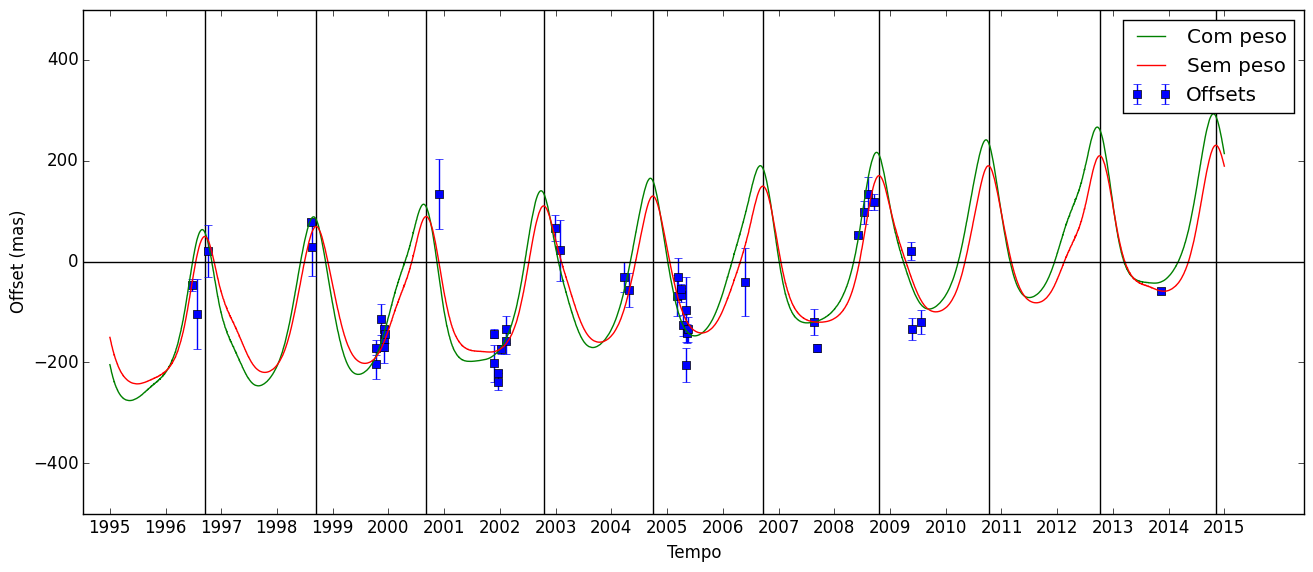
\includegraphics[scale=0.25]{figures/DEC.png}\label{Fig:offxtime}
\caption{Offsets of the declination of Carme by time. \textcolor{red}{Figura só para visualização, vou colocar alguma melhor depois}}
\end{centering}
\end{figure}

\begin{figure}
\begin{centering}
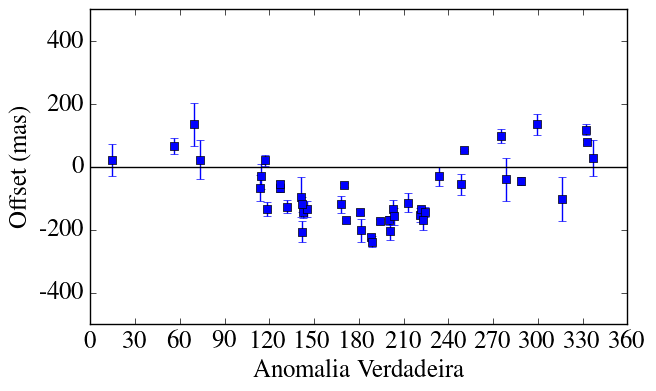
\includegraphics[scale=0.25]{figures/DEC_anom.png} \label{Fig:offxtanom}
\caption{Offsets of the declination of Carme by true anomaly. \textcolor{red}{Figura só para visualização, vou colocar alguma melhor depois}}
\end{centering}
\end{figure}



\begin{equation}
F(t,f) = p[0]\times \frac{t - jd_{0}}{365.65} + p[1]\times \sin(f) + p[2]\times\cos(f) + p[3],
\label{eq:linear}
\end{equation}

\begin{equation}
\begin{split}
%F = \{F_{x} \in  F_{c} &: (|S| > |C|) \\
% &\quad \cap (\text{minPixels}  < |S| < \text{maxPixels}) \\
% &\quad \cap (|S_{\text{conected}}| > |S| - \epsilon) \}
F(t,f) = p[0]\times\sin\left(\frac{2\pi}{p[1]}\times \frac{t - jd_{0}}{365.25} + p[2]\right) + p[3]\times\sin(f) + \\ +p[4]\times\cos(f) + p[5],
\end{split}
\end{equation}



\section{Prediction of occultations} \label{Sec: predictions}

%The prediction of the occultations was made by crossing the stellar coordinates and proper motions of the UCAC4 catalogue \citep{Zacharias2013} with the corrected JPL ephemeris as presented in the section \ref{Sec: Offset}. 


\section{Occultation tests} \label{Sec: testes}

\begin{figure*}
\begin{centering}
\subfigure[Sem offsets]{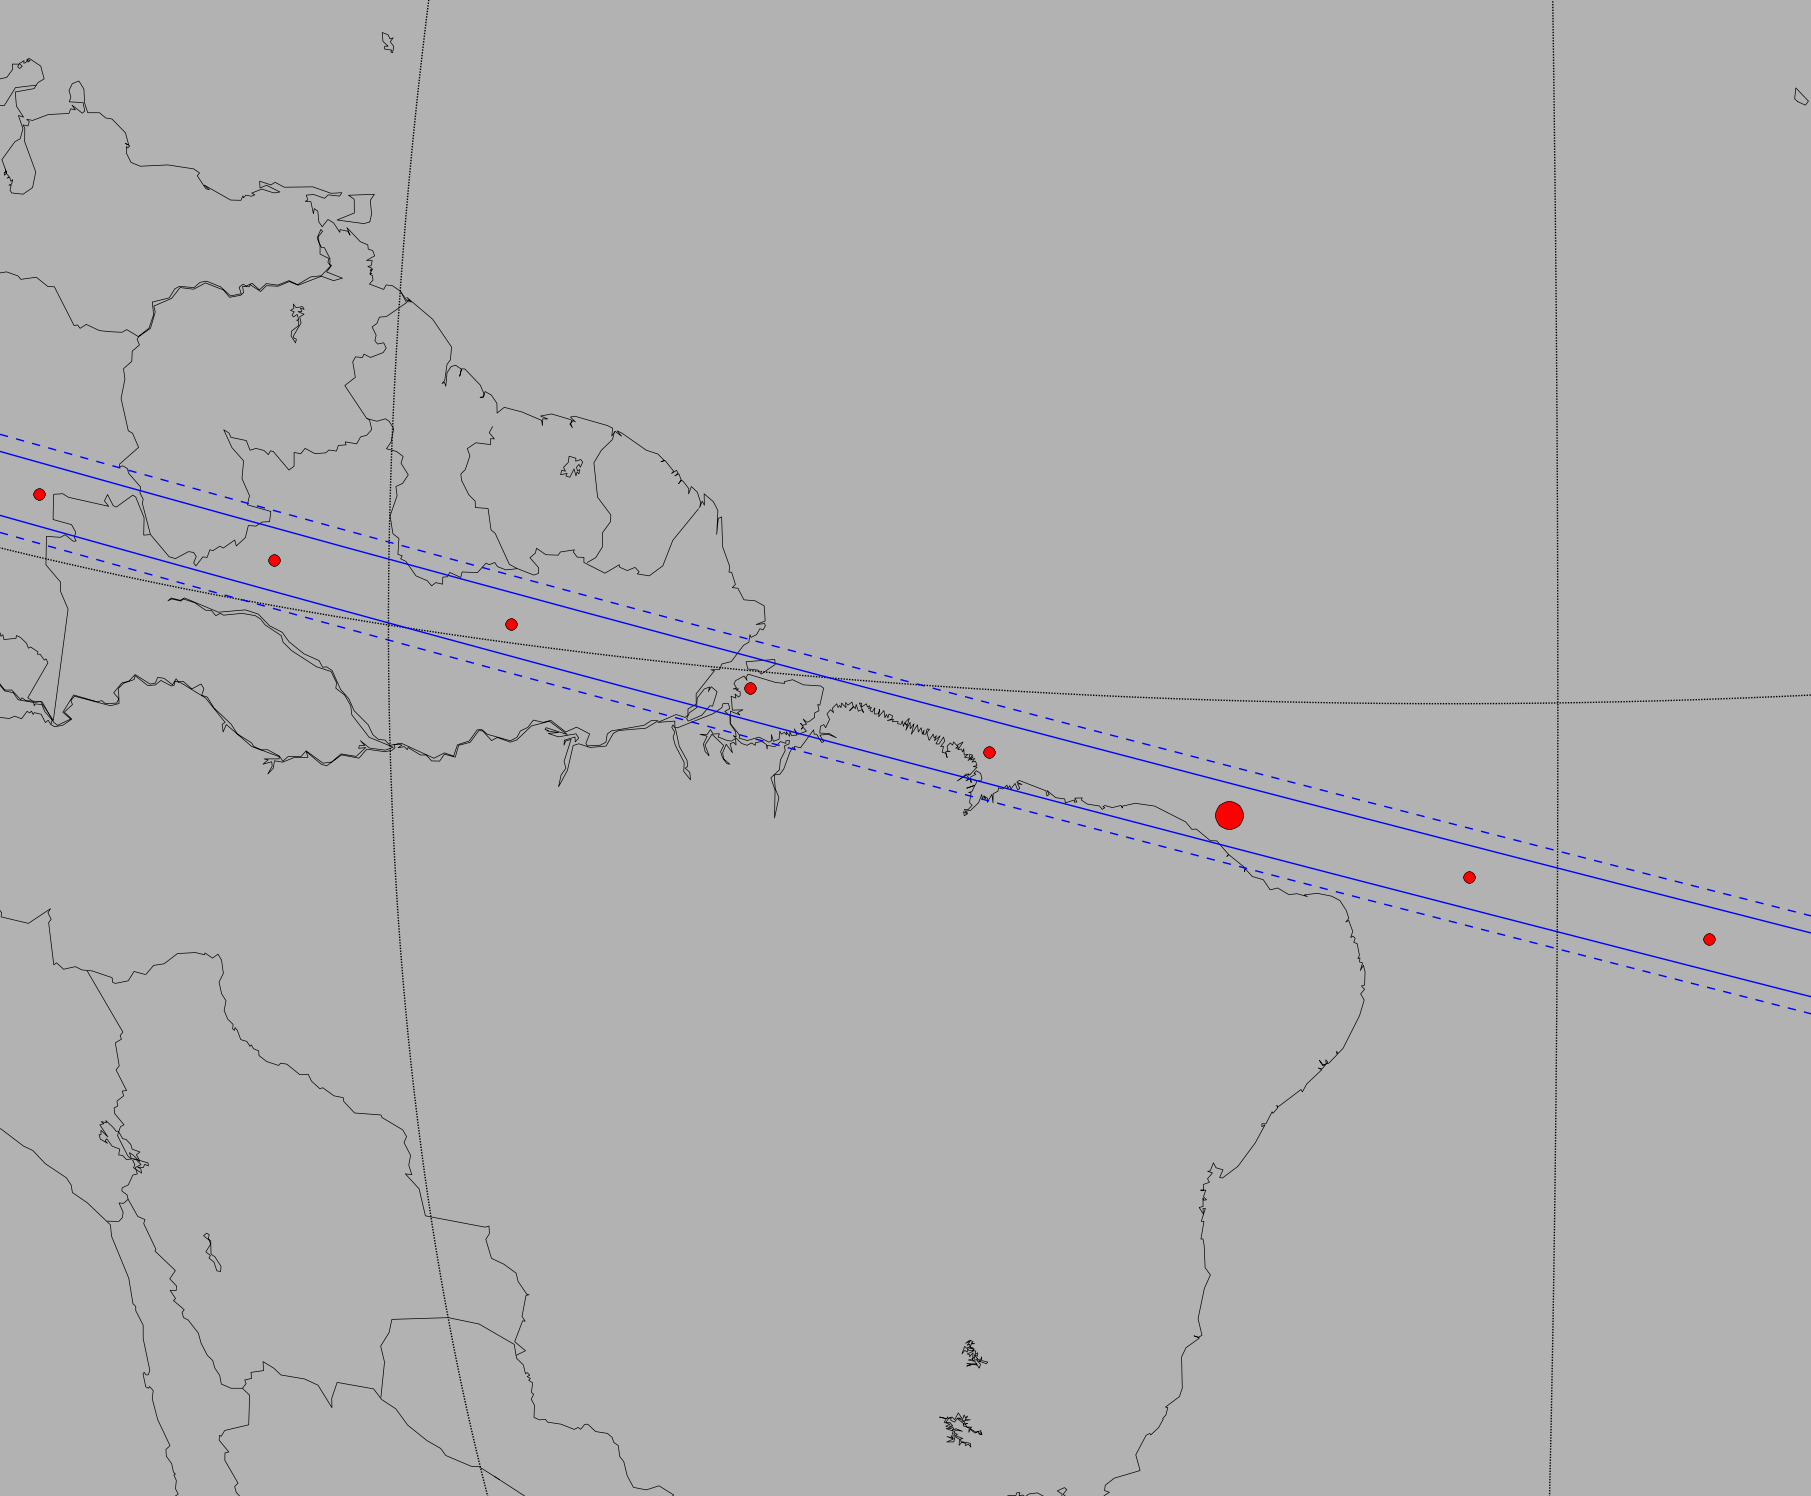
\includegraphics[scale=0.19]{figures/Himalia1_2015-03-03T00:39:25.png}  \label{Fig: occ-Himalia-nooff}}
\subfigure[Offset de Himalia a partir do ajuste]{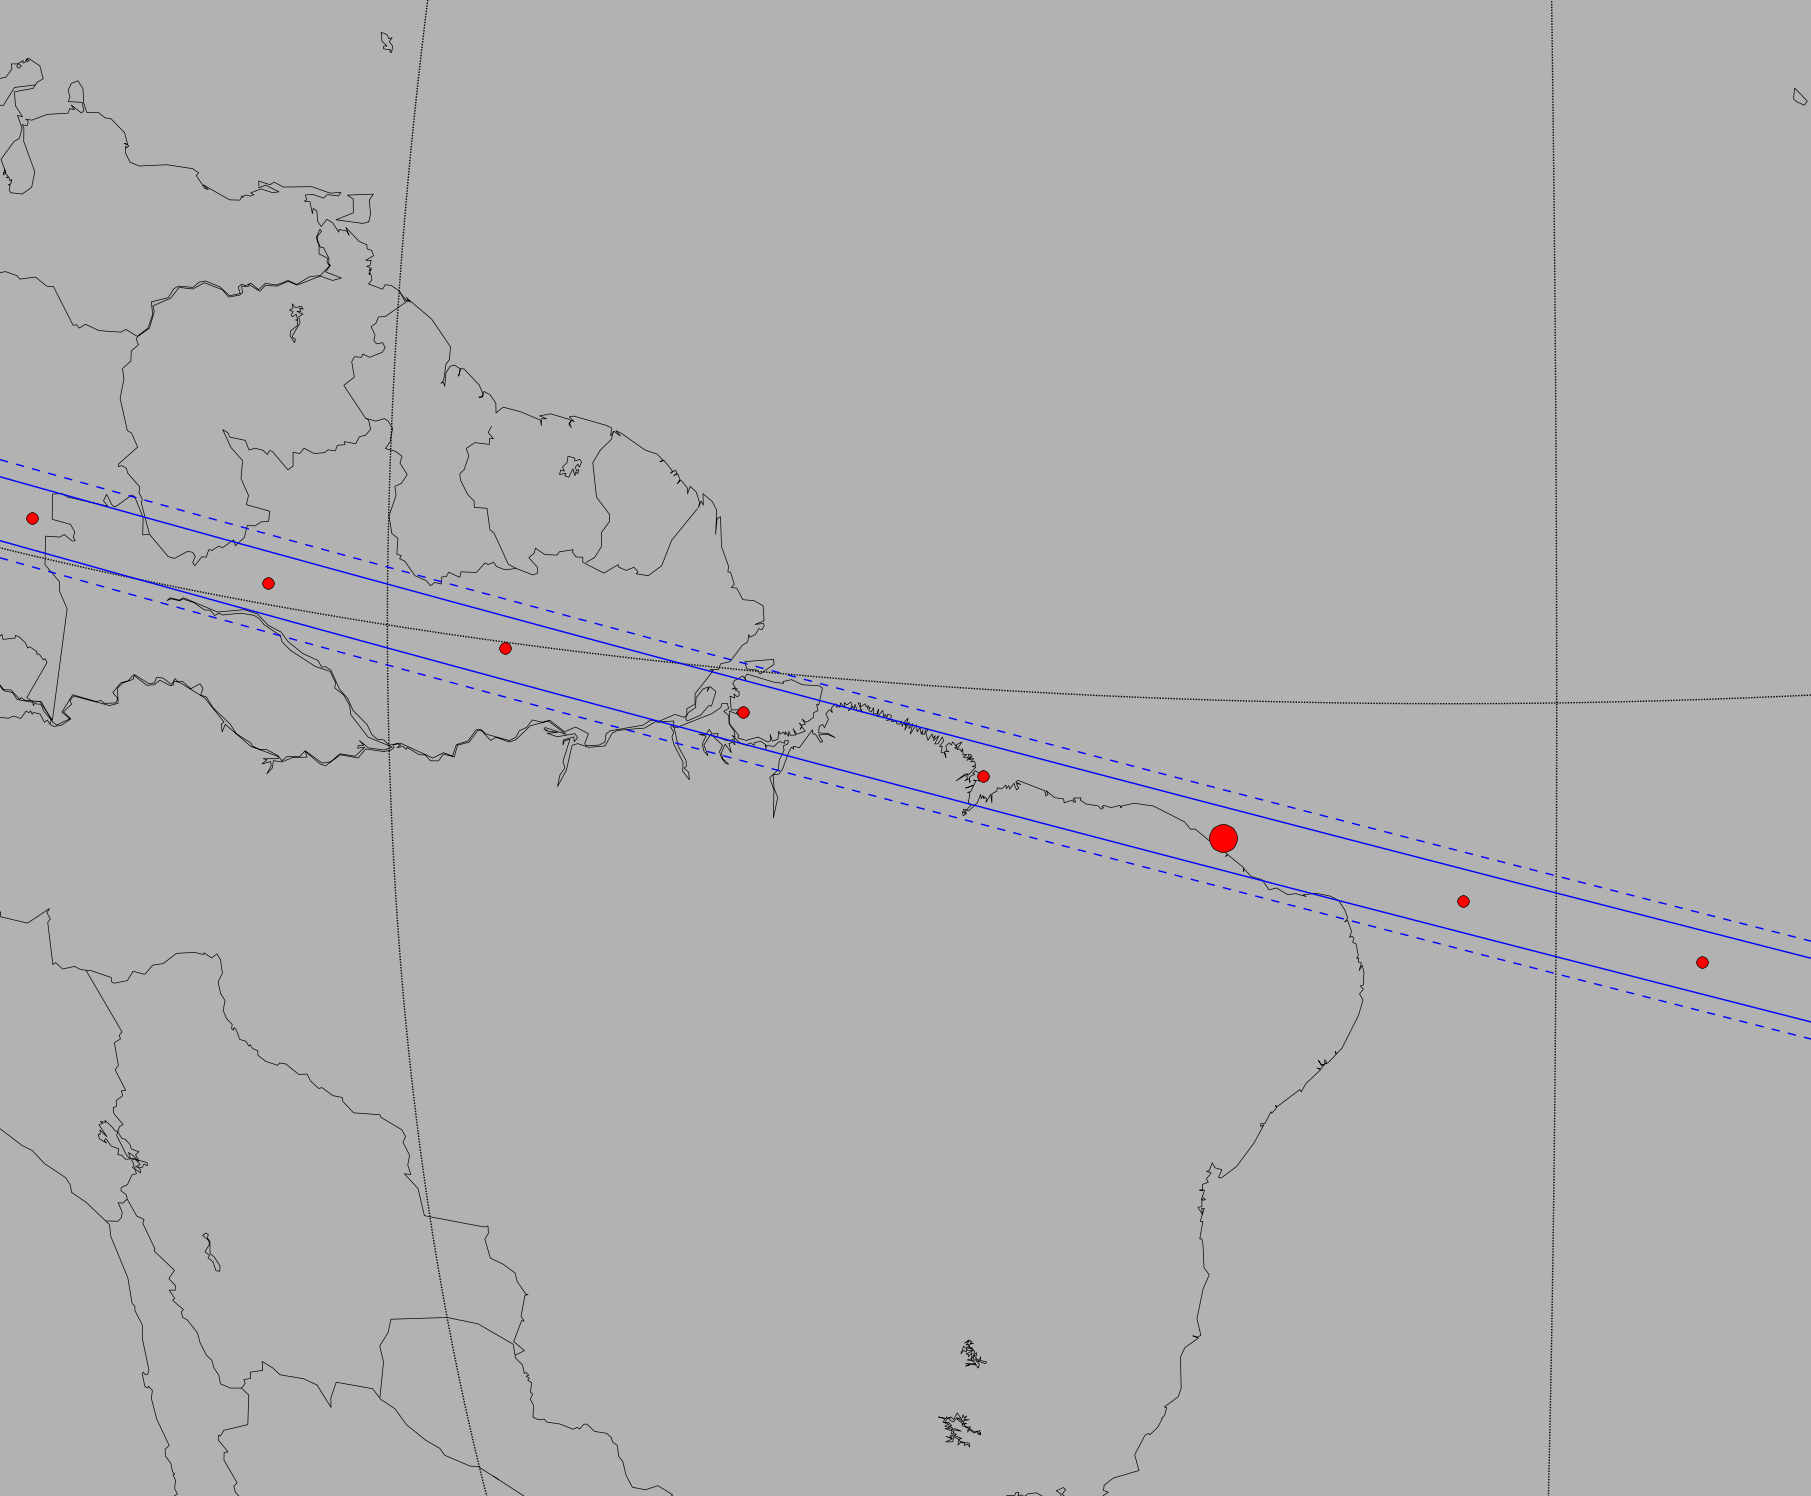
\includegraphics[scale=0.19]{figures/Himalia2_2015-03-03T00:39:18.png}  \label{Fig: occ-Himalia-ajuste}}
\subfigure[Obs. dia 22 de Fevereiro (campos separados)]{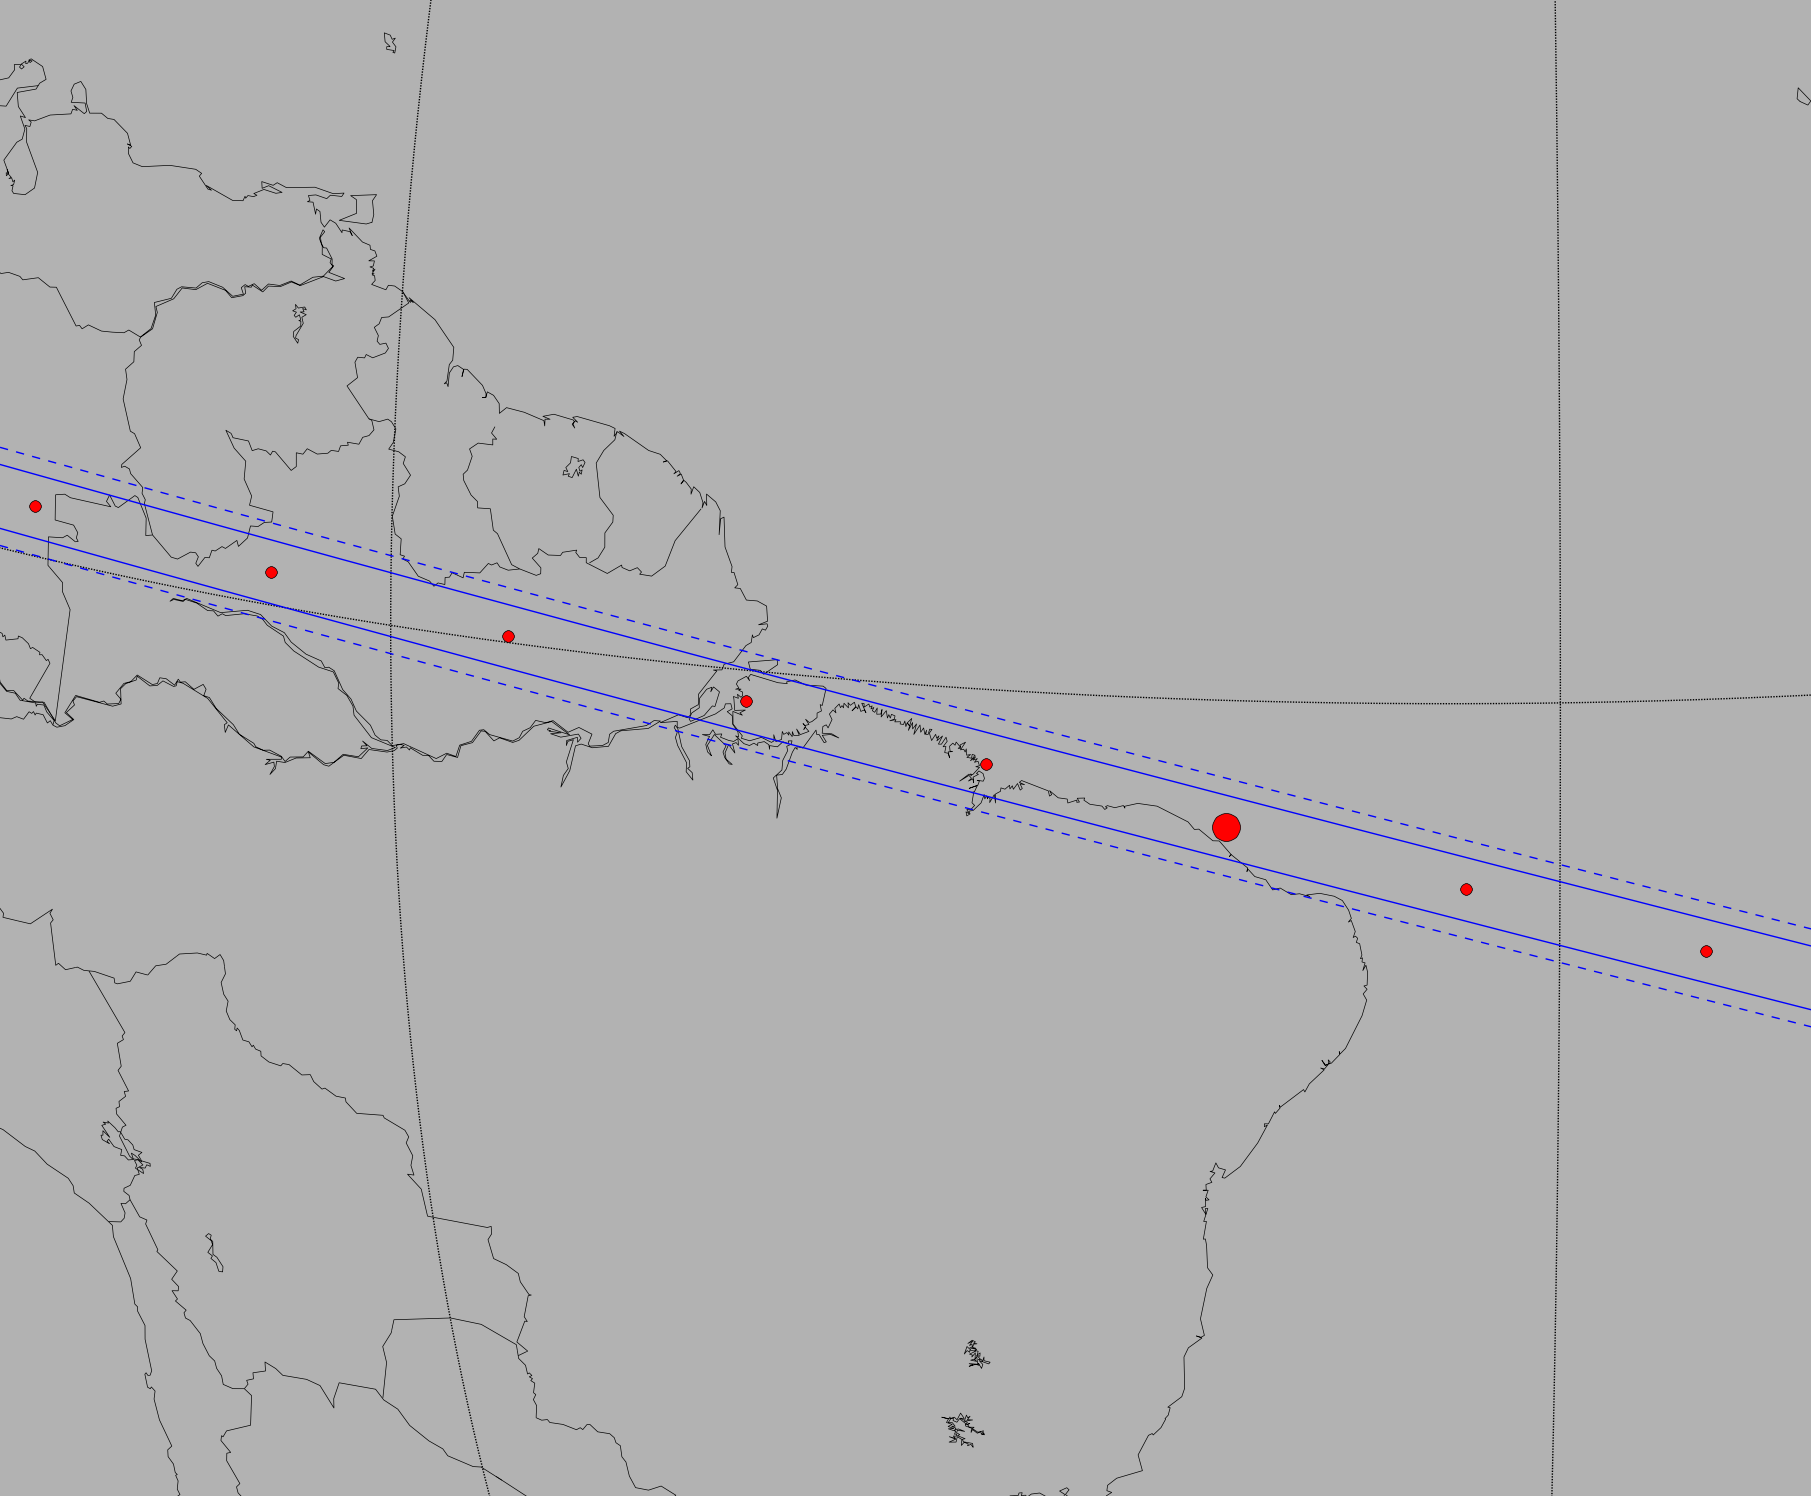
\includegraphics[scale=0.19]{figures/Himalia3_2015-03-03T00:39:40.png}   \label{Fig: occ-Himalia-off22fev}}
\subfigure[Obs. dia 03 de Março (mesmo campo)]{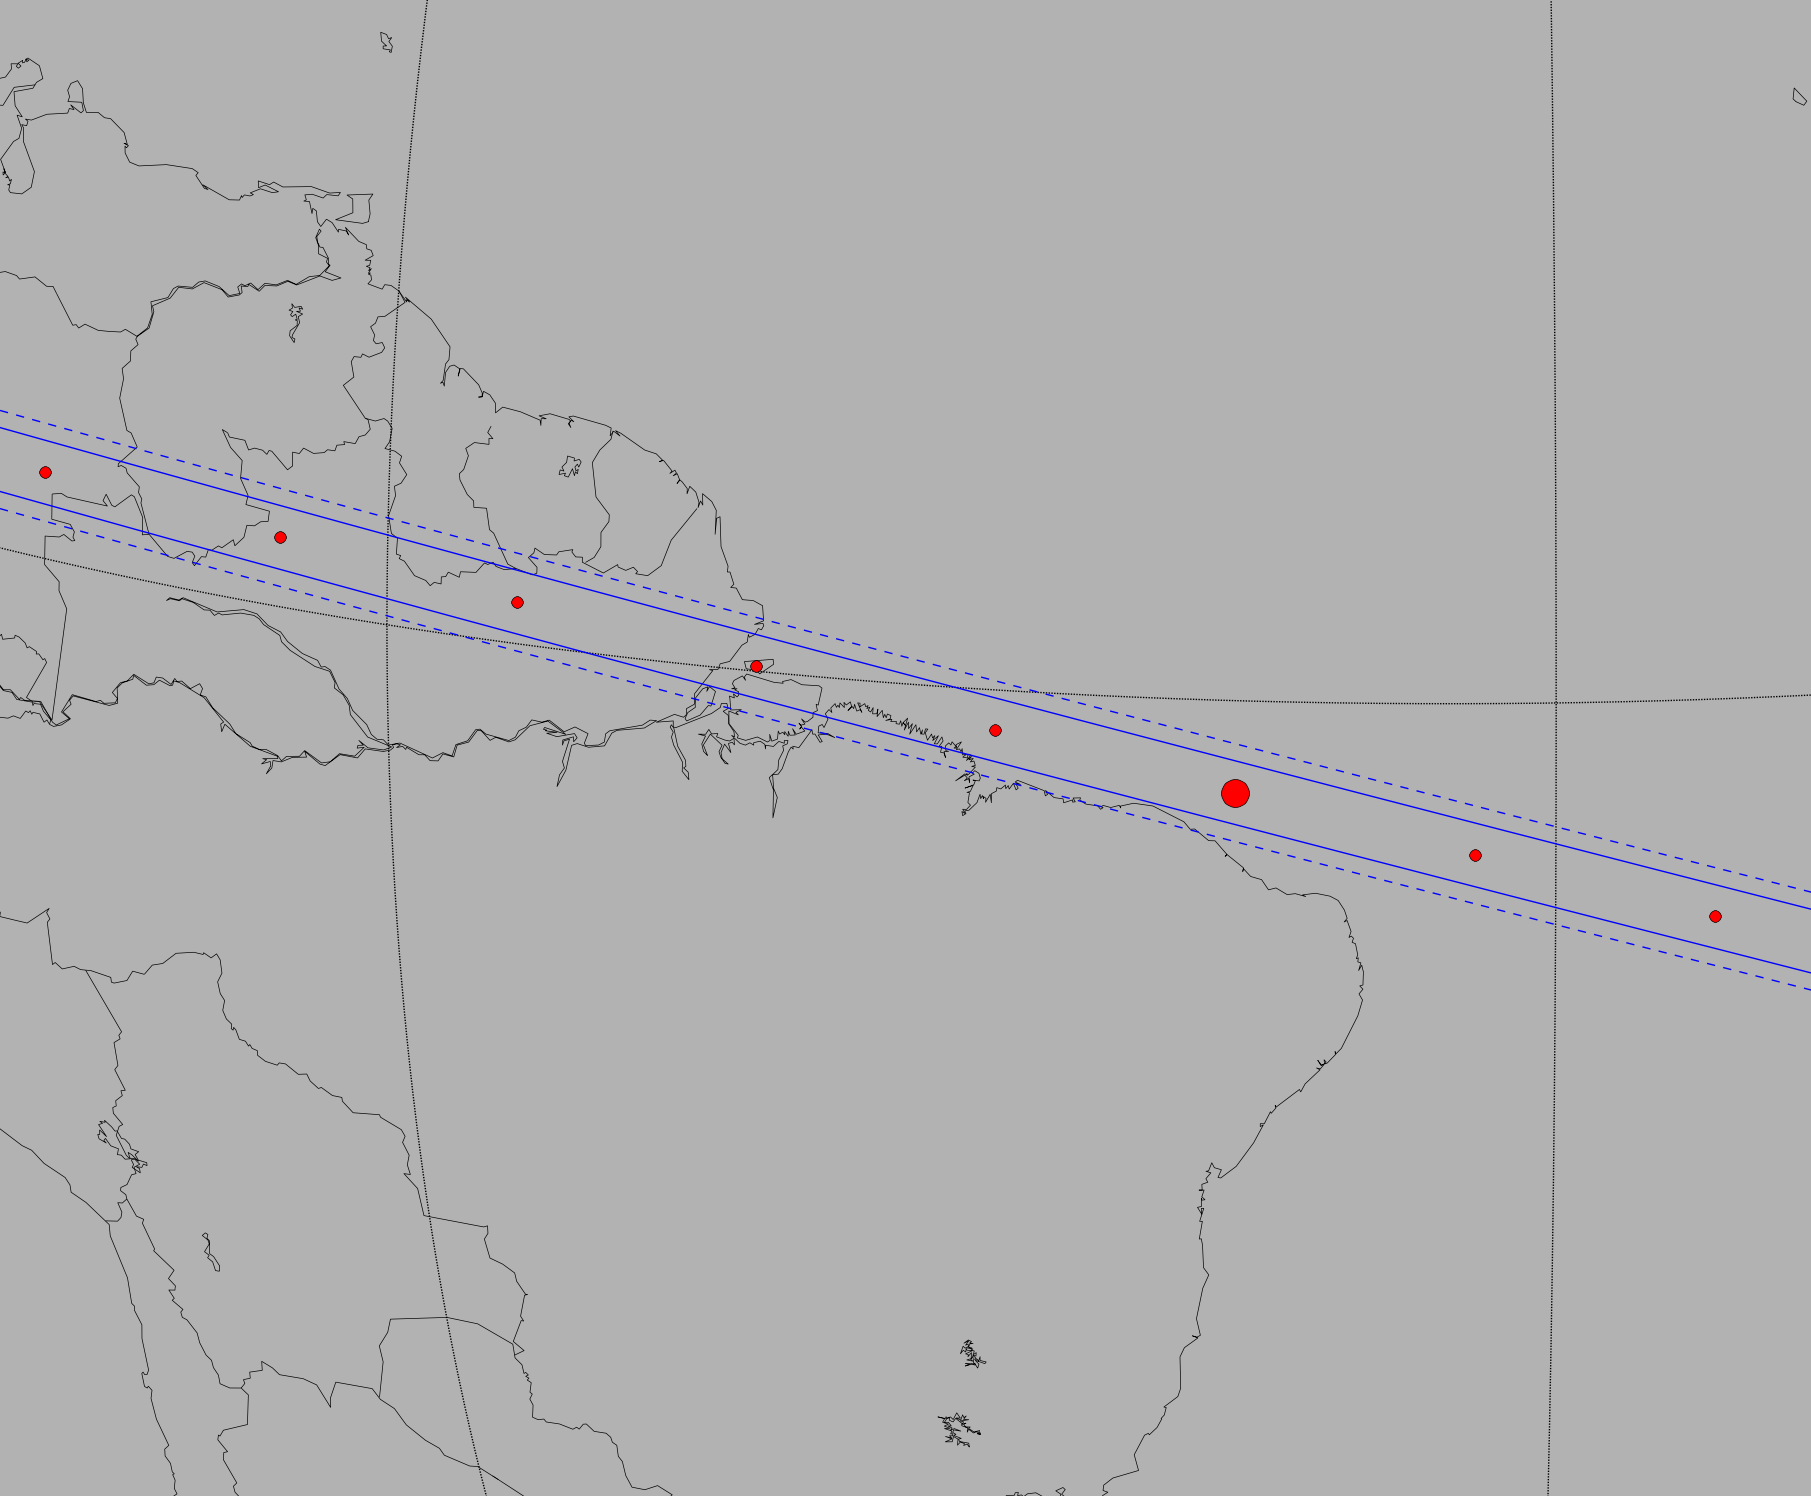
\includegraphics[scale=0.19]{figures/Himalia4_2015-03-03T00:39:15.png}   \label{Fig: occ-Himalia-off03mar}}
\caption{Predictions for Himalia: O ponto grande em vermelho mostra o ponto de máxima aproximação geocêntrica da sombra na Terra, os pontos vermelhos menores são os centros da ocultação separados por um minuto, as linhas retas são os limites das sombras dado o tamanho estimado do objeto e as linhas tracejadas equivalem a uma diferença de 40 mas do centro da sombra representando o erro estimado da predição. (a) é o mapa utilizando apenas as posições nominais da estrela e do satélite. (b) mostra a sombra dado um offset estimado para a posição de Himalia dada sua anomalia verdadeira segundo um ajuste feito em cima dos offsets de efeméride encontrados em \cite{GomesJunior2015-Irregular}. Em (c) são aplicados offsets às posições da estrela e do satélite a partir de observações feitas em 22 de Fevereiro no telescópio Zeiss. Em (d), temos o mesmo que para (c) porém com offsets obtidos de observações feitas em 03 de Março no telescópio Perkin-Elmer quando os objetos estavam próximos no campo.\textcolor{red}{Figuras e texto ainda serão mudados. Colocado para visualização}}
\label{Fig: occ-Himalia}
\end{centering}
\end{figure*}

\section{Conclusion} \label{Sec: conclusions}

%We managed a large database with FITS images acquired by 5 telescopes in 3 sites between 1992 and 2014. From that, we identified 8466 observations of irregular satellites, from which we managed to obtain 6523 suitable astrometric positions, giving a total of 3666 positions for 12 satellites of Jupiter, 1920 positions for 4 satellites of Saturn, 35 positions for Sycorax (Uranus) and 902 positions for Nereid (Neptune).

%The positions of all the objects were determined using the PRAIA package. The package was suited to cope with the huge amount of observations and the task of identifying the satellites within the database. PRAIA tasks were also useful to deal with the missing or incorrect coordinate and time stamps present mostly in the old observations.The UCAC4 was used as the reference frame. Based in the comparisons with ephemeris, we estimate that the position errors are about 60 mas to 80 mas depending on the satellite brightness.

%For some satellites the number of positions obtained in this work is comparable to the number used in the numerical integration of orbits by the JPL \citep{Jacobson2012} (see Table \ref{Tab: comparison-horizons}). For instance, the amount of new positions for Himalia is about 70\% of the number used in the numerical integation of orbits by JPL. Systematic errors in the ephemeris were found for at least some satellites (Ananke, Carme, Elara and Pasiphae). In the case of Carme, we evidenced an error in the orbital inclination (see Fig. \ref{Fig: carme_anom}).

%The positions derived in this work can be used in new orbital numerical integrations, generating more precise ephemerides. Stellar occultations by irregular satellites could then be better predicted. Based in this work, our group has already computed occultation predictions for the 8 major irregular satellites of Jupiter. These predictions will be published in a forthcoming paper.


\begin{acknowledgements}

ARG-J thanks the financial support of CAPES. MA thanks the CNPq (Grants 473002/2013-2 and 308721/2011-0) and FAPERJ (Grant E-26/111.488/2013). RV-M thanks grants: CNPq-306885/2013, Capes/Cofecub-2506/2015, Faperj/PAPDRJ-45/2013. JIBC acknowledges CNPq for a PQ2 fellowship (process number 308489/2013-6). FB-R acknowledges PAPDRJ-FAPERJ/CAPES E-43/2013 number 144997, E-26/101.375/2014. BEM thanks the financial support of CAPES.

\end{acknowledgements}

\bibliographystyle{aa}
\nocite{*}
\bibliography{references.bib}


\end{document}
